\hspace{4.5mm}
O relatório destaca as reuniões realizadas pela equipe de projeto e os avanços feitos ao longo das etapas de planejamento, ação, revisão e correção. Nas primeiras reuniões, a equipe ainda estava se familiarizando com as ferramentas a serem usadas, como Git, Figma e o Overleaf, enquanto aguardava uma entrevista com o cliente para cobrir alguns poucos pontos que ficaram faltando para o esclarecimento das funcionalidades do sistema. Houve a ausência de alguns membros nas primeiras sessões, como Maria Luísa e Henrique, e a gravação da primeira reunião foi corrompida, o que gerou dificuldades de comunicação. O Scrum Master tomou providências para enviar um resumo em áudio e abriu um repositório Git para facilitar a colaboração entre os membros.
\par
Com o avanço das semanas, novas tarefas foram iniciadas, como o estudo de viabilidade, a definição do problema e do objetivo do projeto, e o desenvolvimento da identidade visual. No entanto, problemas de comprometimento continuaram, o que afetou diretamente o progresso. Algumas tarefas essenciais foram concluídas, como o estudo de Git e a coleta dos perfis do GitHub dos participantes, além da definição clara do cliente e dos objetivos do projeto. Das definições da parte de implementação, o backend foi atribuído a Guilherme e Vinícius, enquanto o frontend ficou sob a responsabilidade de Lucas e Maria Luísa. Também foi enfatizado que todas as colaborações seriam melhor aproveitadas se fossem ativamente expostas para os outros membros por meio de reuniões online para confecção dos artefatos.
\par
Nas reuniões mais recentes, o foco, além da revisão e correção dos atributos que foram iniciados, passou a ser a conclusão dos requisitos funcionais e não funcionais, além da elaboração do termo de aceite. O time também começou a trabalhar no Figma para a criação das telas, apesar de atrasos causados pela ausência do Scrum Master na coordenação e agendamento dessas reuniões específicas para o desenvolvimento de um artefato. Membros como Lucas não contribuíram com o projeto, mesmo após várias tentativas de contato, e Vinícius teve problemas de saúde e de sua vida profissional que o afastaram temporariamente. Mesmo com esses desafios, a equipe avançou na revisão dos artefatos e está se preparando para a apresentação final do projeto, agendada para o dia 27 de setembro, com Evellyn e Vinícius encarregados da apresentação.
O documento completo do relatório se apresenta na próxima página, e se estende até as 3 páginas seguintes.
\includepdf[pages=2-]{./PDFs/Relatorio_PS.pdf}